\documentclass[a4paper,12pt]{article}

\usepackage{graphicx} % Required for inserting images
\usepackage[utf8]{inputenc}
\usepackage[english]{babel}
\usepackage[letterpaper,top=2cm,bottom=2cm,left=3cm,right=3cm,marginparwidth=1.75cm]{geometry}
\usepackage{tocloft}    %necessario per inserire i puntini nell'indice
\usepackage{url}    %necessario per i collegamenti ipertestuali
\usepackage[nottoc]{tocbibind}  %necessarrio per far apparire la bibliografia nell'indice
\usepackage{verbatim} %serve per commentare più righe contemporaneamente
\usepackage{endnotes}





\title{How artificial intelligence has transformed the school education sector}
\author{Alessandro Castelli \and ID: 12246581}
\date{\today}

\begin{document}    %inizio documento

\maketitle  %Creo il titolo
\thispagestyle{empty}   %Non metto il numero di pagina nel frontespizio
\pagebreak  %Inserisco interruzione

\cftsetpnumwidth{0.5cm} %distanza puntini da numero
\renewcommand{\cftsecdotsep}{4} %densita di puntini
\tableofcontents    %Inserisco indice


\setcounter{page}{1}    %Inizio a contare da 1
\newpage    %Altra pagina

\section{Introduction}  %Creo la sezione Introduzione
Since the second half of the 1990s, humanity has started questioning the concept of artificial intelligence. In the subsequent years, significant progress has been made in this field, thanks to numerous discoveries. One of the most renowned artificial intelligence systems is \textbf{ChatGPT}, a software designed to simulate conversations with human beings. It operates based on GPT-3, a natural language processing model developed by OpenAI\footnote{Readily available: https://openai.com/chatgpt}. With its 175 billion parameters, it stands as one of the most versatile models in its category.

Other lesser-known but widely used systems in the field we are discussing include:
\begin{itemize}
    \item \textbf{ALEKS}: ALEKS (Assessment and Learning in Knowledge Spaces) is an intelligent tutoring system that adapts to students' learning levels and provides a personalized learning path in various subjects\footnote{Readily available: https://www.aleks.com/}.
    \item \textbf{Carnegie Learning}: Carnegie Learning is a company that develops AI-based mathematics software. Their programs use AI to monitor students' progress, provide feedback, and adapt exercises to their needs\footnote{Readily available: https://www.carnegielearning.com/}.
    \item \textbf{Cognii}: Cognii is an AI specialized in natural language analysis and text processing. It is used to provide immediate and personalized feedback to students on their written responses\footnote{Readily available: https://www.cognii.com/}.
\end{itemize}
\begin{comment}
Fin dalla seconda metà degli anni 90 del secolo precedente l'umanità ha inziato ad interrogarsi sul concetto di intelligenza artificiale.Negli anni seguenti grazie alle innumerevoli scoperte in quel campo sono stati fatti grandi progressi.\\Uno dei sistemi di intelligenza artificale più famosi è ChatGPT, un software progettato per simulare una conversazione con un essere umano. Il suo funzionamento si basa su GPT-3, un modello di elaborazione del linguaggio naturale sviluppato da OpenAI. I suoi 175 miliardi di parametri lo rendono uno dei modelli più versatili della categoria.

Altri sistemi meno famosi ma che sono molto utilizzati nell'ambito che tratteremo sono :
Watson Education: Sviluppato da IBM, Watson Education è un'IA che offre strumenti per la personalizzazione dell'apprendimento, l'analisi dei dati degli studenti e l'assistenza nella valutazione degli apprendimenti.

ALEKS: ALEKS (Assessment and Learning in Knowledge Spaces) è un sistema di tutoraggio intelligente che si adatta al livello di apprendimento degli studenti e fornisce un percorso di apprendimento personalizzato in vari argomenti.

Carnegie Learning: Carnegie Learning è un'azienda che sviluppa software di matematica basato sull'intelligenza artificiale. I loro programmi utilizzano l'IA per monitorare il progresso degli studenti, fornire feedback e adattare gli esercizi alle loro esigenze.

Cognii: Cognii è un'IA specializzata nell'analisi del linguaggio naturale e nell'elaborazione del testo. Viene utilizzata per fornire feedback immediato e personalizzato agli studenti sulle loro risposte scritte.
\end{comment}


\subsection{What you will find}
In the following essay, you will initially find an introduction on how technology, throughout the centuries, has been gradually introduced into educational environments. Subsequently, I will focus on how artificial intelligence systems have started to play a central role in the field of education. Finally, I will attempt to analyze the positive and negative aspects of using these systems in the education of young students.
\begin{comment}
Nel seguente elaborato troverai inizialmente un'introduzione su come la tecnologia, attraverso i secoli, sia stata gradualmente introdotta negli ambienti educativi, successivamente mi concentrerò su come i sistemi di intelligenza artificiale hanno iniziato ad avere un ruolo centrale in ambito educazionale ed infine  cercherò di analizzare i lati positivi e negativi dell'uso di questi sistemi nell'educazione dei giovani ragazzi.
\end{comment}


\section{Technology and Education through the centuries}
Technology and education have been interconnected for many centuries. Throughout history, humanity has utilized tools that enable more effective studying for students. For instance, rulers were used to facilitate precise measurements in geometry, abacuses simplified mathematical operations, and the invention of paper revolutionized the dissemination of knowledge. With the advent of the digital age, numerous other technological innovations have been introduced, many of which are still used today. For example, calculators facilitate mathematical operations, radios provide real-time information, televisions enable education through digital content, and finally, computers have transformed the educational landscape.

\begin{comment}
    Tecnologia ed educazione sono legati ormai da molti secoli. 
    L'umanità ha sempre usato strumenti che permettevano allo studente di studiare in maniera più efficace. 
    Si pensi per esempio ai righelli che permettevano di fare misurazioni più efficaci nella materia della geometria, agli abachi che semplificavano le operazioni matematiche, all'invenzione della carta etc. 
    Con l'avvento del digitale sono state introdotte moltre altre innovazioni tecnologiche molte delle quali vengono usate anche ai nostri giorni. 
    Per esempio: la calcolatrice che permette di fare operazioni matematiche, la radio che permette l'informazione in tempo reale, la televione che permette l'educazione attraverso contenuti digitali ed infine il computer.
\end{comment}

\subsection{Computer}
Computers have seen increasingly widespread use since their invention. The arrival of computers and, subsequently, the Internet has forever changed the field of education. 
It has become possible to utilize increasingly sophisticated software that allows students to delve deeper into subjects and access information more easily and quickly.
Another significant turning point was the introduction of portable electronic devices such as tablets, notebooks, smartwatches, and so on. 
Thanks to their lightweight nature, it has become feasible to carry these devices anywhere, including classrooms during lessons.
This implies that from a certain point onward, computers have not only been an additional tool to be used at home but also a fully-fledged educational instrument that has become an integral part of students' lessons.
\begin{comment}
    I computer hanno avuto un uso sempre maggiore dalla loro invenzione. 
    La venuta prima dei computer e poi di Internet ha per sempre cambiato il mondo dell'insegnamento. è stato possibile ustilizzare software sempre più elaborati che permettono allo studente un maggiore approfondimento ed una maggiore facilità nel reperire l'informazione in tempo breve.
    Un altro grande punto di svolta è stato l'introduzione dei dispositivi eletrronici portatili come: tablet, notebook, smartwatch, etc.
    Data l'estrema leggerezza di questi dipositivi è statopossibile portarli ovunque quindi anche in classe durante le lezioni.
    Questo implica il fatto che da un certo punto in poi i computer non sono stati soltanto uno strumento in più da utilizzare a casa ma anche uno strumento didattico a tutti gli effetti che sono entrati a far parte delle lezioni dello studente.
\end{comment}


\section{AI systems used in educational contexts}
Artificial intelligence systems have been a natural progression from the use of software devices in schools. In the following section, we will analyze the potential uses of this technology both by students and teachers.
\\ \newline

\begin{comment}
    I sistemi di Intellgenza artificiale sono stati il naturale sviluppo dell'utillo di dispositivi software nella scuola. Nella sezione seguente saranno analzzati i possibili usi di questa tecnologia sia da parte dello studente che da parte dell'insegnante.

\end{comment}

\subsection{Artificial Intelligence and teachers}
Artificial intelligence systems can be very useful not only for students but also for teachers. AI can help reduce unproductive time during lessons. For example, it can be used to automatically update the attendance register of students in the classroom by utilizing computer vision systems \cite{dimitriadou2023critical}.

Furthermore, AI can assist teachers in identifying students who are not paying much attention in class. This way, they can be called upon by the teacher and included in the normal course of a lesson. It can also be helpful in recognizing symptoms of illnesses in students with specific disorders, allowing teachers to provide timely assistance. For instance, it can help identify an epileptic seizure in students suffering from epilepsy\cite{dimitriadou2023critical}.

Lastly, AI can support teachers for the classroom management, in other word AI help the teacher in lesson planning and the development of personalized study plans for each student based on their individual needs.
\begin{comment}
    I sistemi di intelligenza artificiale possono essere molto utili non solo agli studenti ma anche agni insegnanti. 
    AI  può essere utile per ridurre i tempi non utili durante le lezioni per esempio può essere usato per aggiornare in automatico il registro delle presenze degli studenti in aula (utilizzando sistemi di computer vision[4].
    Inoltre può aiutare l'insegnante nel riconoscimento degli studenti che non prestano molta attenzione in classe, in questo modo possono essere richimati dall'insegnante ed inclusi nel normale svolgimento di una lezione, può essere utile nel riconoscere sintomi di malattie negli studenti con particolari disturbi, in questo modo gli insegnati potranno soccorrerli in tempo (per esempio riconoscere un attacco epilettico negli studenti che soffrono di epilessia), infine può aiutare l'insegante nella programmazione delle lezioni e nella compilazione di piani di studio personalizzati per ogni alunno in base alle sue necessità.
    
\end{comment}

\subsection{Artificial intelligence and students}
In recent years, numerous international experiments have been conducted where Artificial Intelligence has been used in the field of education. It can be utilized both as a subject to study and as a tool to use\cite{cesaretti2021intelligenza}. 
In our analysis, we will focus on the second aspect.

In Figure \ref{fig:enter-label}, you can see the main scenarios of artificial intelligence in students' lives and the technologies supporting these scenarios.
\begin{figure}
     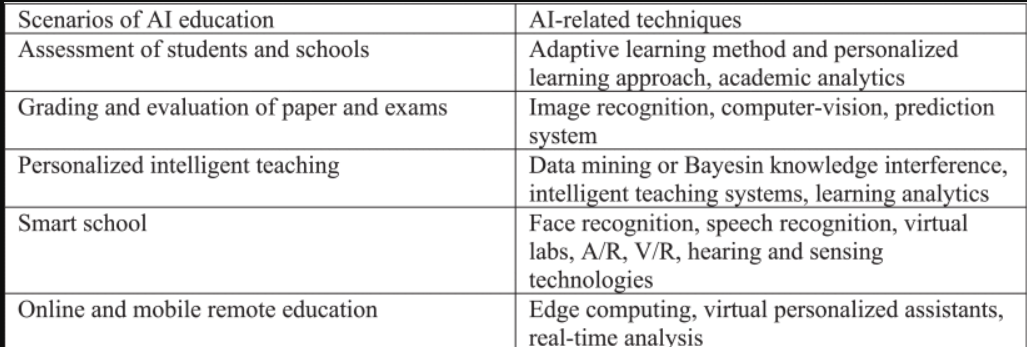
\includegraphics[scale=0.8]{figure1.png}
     \caption{Techniques for Scenarios of AI Education \cite{ArtificialInInEd}}
     \label{fig:enter-label}
 \end{figure}
\begin{comment}
    In questi ultimi anni innumerevoli sono state le sperimentazioni internazionali in cui l’Intelligenza Artificiale è stata utilizzata in campo educativo. Essa può essere utilizzata sia come argomento da studiare sia come stumento da usare.
    Noi ci concentremo sul secondo aspetto.

    Nella  figura Figure1 seguente potrai vedere i principali scenari dell'intelligenza artificiale nella vita degli studenti e le tecnologie a supporto di questi scenari.
    
\end{comment}

\subsubsection{Artificial Intelligence as a tutor}
In some articles\cite{aleven2009new}, it is explained how: \begin{quote}
\textit{
    "Intelligent tutoring systems draw on artificial intelligence technology to provide interactive instruction that adapts to individual students’ needs and, most typically, supports student practice in learning complex problem-solving and reasoning"}
\end{quote}
Many studies have shown that some artificial intelligence systems are capable of selecting tasks that are at the level of the selected student and on which the student can work without too much difficulty, while still learning new information. This is made possible through the dialogue between the user and the artificial intelligence system, as well as natural language processing techniques. This technique can improve the quality of education for every student because it can create personalized adaptive content tailored to the needs and learning abilities of each student.
\begin{comment}
    In alcuni articoli viene spegato come ....cit...
    Sono stati fatti molti studi che mostrano come alcuni sistemi di intelligenza artificiale siano capaci di selezionare compiti che siano al livello dello studente selezionato e su cui lo  studente può lavorare senza troppe difficoltà ma comunque imparando nuove informazioni. Questo è possibile grazie a dialogo tra utente e Intelligenza artificiale e tecniche di elaborazione del linguaggio naturale. Questa tecnica può quindi migliorare la qualità dell'istruzione di ogni studente perchè riesce a creare contenuti adattivi personalizzati per le esigenze e le capacità di apprendimento di ogni studente.
\end{comment}

\begin{figure}
    \centering
    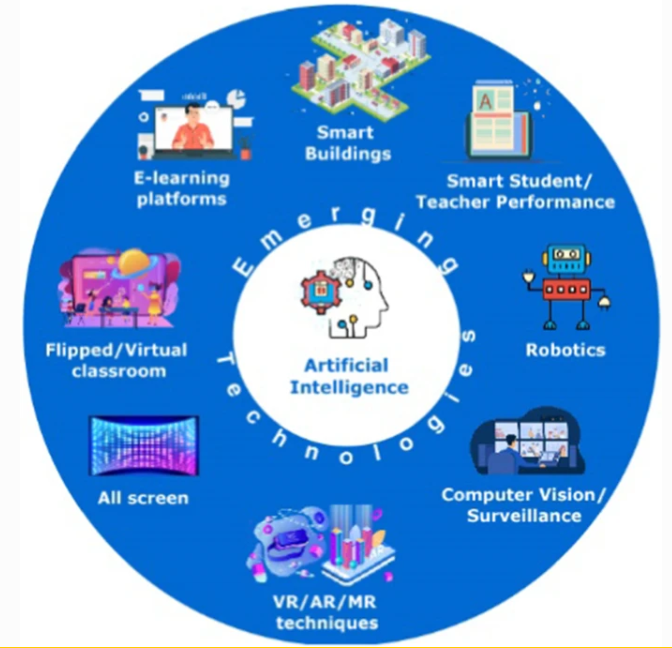
\includegraphics[scale=0.5]{figure2.png}
    \caption{The main technologies present in a smart classroom \cite{dimitriadou2023critical}}
    \label{fig:enter-label2}
\end{figure} 

\subsubsection{Artificial Intelligence and smart classroom}
We can define a smart classroom as an environment where the physical and digital spaces are seamlessly integrated. These classrooms are equipped with advanced technologies such as projectors, interactive whiteboards, advanced software, etc., as depicted in Figure \ref{fig:enter-label2} which make the environment engaging. These classrooms enable improved performance, creative thinking, and enhanced student outcomes.
In recent years, smart classrooms have increasingly integrated with artificial intelligence systems. By utilizing this technology, a significant advancement in teaching can be achieved. It enables the creation of original digital content that can be directly used in the classroom, as well as almost real-time automatic evaluation of exercises completed by students to assess their level of knowledge in a subject.
Furthermore, smart classrooms often feature robots that are increasingly integrated with artificial intelligence systems, providing an enjoyable learning experience for students.


\begin{comment}
    Possiamo definire una smartclassroom come un ambiente in cui l'ambiente fisico e quello digitale sono perfettamente integrati. In queste aula sono presenti molte tecnologie avanzate come proiettori, lavagne multimediali, software avanzati, etc, come puoi vedere in figura 2.  che rendono l'ambiente stimolante. Queste classi permettono di migliorare le prestazioni, il pensiero creativo e le performance degli studenti.

    Nel corso degli ultimi anni le smartclasroom si sono sempre più integrate con i sistemi di intelligenza artificiale. Utilizzando questa tecnolgia è possibile fare un grande passo avanti nellìinsegamento, infatti  è possibile la creazione di contenuti digitali originali usufruibili direttamente in aula è valutazione automatica quasi in tempo reale di esercizi svolti dallo studente per verificare il proprio grado di conoscenza su una materia.


    Inoltre spesso nelle smartclassroom sono presenti robot che sono sempre più integrati con sistemi di intelligenza artificiale insiemi a quali lo studente può imparare divertendosi.
    
\end{comment}

\subsubsection{Artificial intelligence and the study of languages}
Another area of recent development in the education sector is the teaching of new languages through artificial intelligence systems. AI systems, especially chatbots, can assist students in several ways. Here are some of them\cite{haristiani2019artificial}:
\begin{itemize}
    \item Students tend to feel more relaxed when interacting with a bot compared to speaking with a person.
    \item Bots can repeat the same topic multiple times, allowing for reinforcement and better understanding.
    \item Bots provide both text and voice synthesis, enabling students to practice both listening and reading skills.
    \item With bots, students can explore and experiment with linguistic structures that they might not otherwise have the opportunity to use.
    \item Bots can provide immediate feedback on the grammatical style used by the student.
\end{itemize}

\begin{comment}
    Un altro ambito in recente svilippo per quanto riguarda il settore educativo è l'insegnamento di nuove lingue attraverso sistemi di intelligenza artificiale. 
    I sistemi di intelligenza artificiale, specialmente i chatbot, possono aiutare gli studenti in diversi modi. Di seguito ne elencherò alcuni: Innanzitutto è emerso che gli studenti tendono a sentirsi più rulassati quando parlano con un bot di quando parlo con un persona. 
    I bot possono ripetere anche molto volte lo stesso argomento.
    I bot forniscono sia testo che sintesi vocali quandi gli studenti si possono esercitare sia sull'asccolta sia sulla lettura.
    Con i bot è possibile utilizzare strutture linguistiche che altrimeni normalmente non si avrebbe modo di utilizzare.
    I bot possono dare riscontri rapidi sullo stile grammaticale usato dallo studente.
    
\end{comment}
\subsubsection{Artificial Intelligence and students with cognitive difficulties}
Another educational field where artificial intelligence is proving to be very useful is in assisting and supporting students with disabilities. AI systems can support these students in various ways, such as providing low-risk environments, facilitating collaborative learning, and reinforcing positive social behavior\cite{salas2022artificial}.
Artificial intelligence systems can be helpful both in diagnosing these issues and in providing assistance to students who have been diagnosed with them\cite{drigas2013review}.

AI can be used not only to support teaching but also to enhance the communication skills of children with autism. It can create learning environments where children diagnosed with autism spectrum conditions engage in simulated social interactions that serve as a "training ground" for real-world social situations they will encounter\cite{porayska2018blending}.



\begin{comment}
    Un altro campo educativo in cui l'intelligenza artificiale si sta rivelando molto utile è nell'ambito dell'aiuto e sostegno a studenti con disabilità.
    I sistemi di intelligenza artificiale possono supportare questi studenti in vari modi come: essi possono fornire ambienti a basso rischio, sostenere l'apprendimento collaborativo e rafforzare il comportamento sociale positivo CIT. 
    Inoltre i sistemi di intelligenza artificiale possono essere utilia sia nella diagnostica di questi problemi sia nell'aiuto agli studenti a cui questi problemi sono stati diagnosticati.

    L'intelligenza artificiale può essere usata non solo per supportare la didattica ma anche le capacità di comunicazioni di bambini affetti da autismo. Essi infatti riescono a creare ambienti di apprendimento in cui i bambini con diagnosi di condizioni dello spettro autistico si impegnano in interazioni sociali simulate che sono usate come "ambiante di addestramento" per le situazioni sociali in cui si troveranno nel mondo reale.
\end{comment}
\section{Concerns with Artificial Intelligence Systems}
In the following section, we will discuss the critical issues associated with the use of artificial intelligence in the educational field.
Defining and analyzing these activities is not a simple task, as these technologies are constantly evolving.
\begin{comment}
Nella sezione seguente si tratteranno i temi critici che porta con sè l'utilizzo dell'intelligenza artificiale in ambito educativo.

Definire ed analizzare queste attività non è un lavoro semplice dal momento che queste tecnologie sono in continua evoluzione.

    -privacy https://www.mdpi.com/1660-4601/19/3/1192
\end{comment}

\subsection{Privacy}
Artificial intelligence systems often require information about the students using them in order to function effectively. The collected information should be limited to what is necessary for the intended purpose, which is training the AI. Educators should also ensure that students understand the consequences of using these technologies\cite{barua2022artificial}. Additionally, the companies producing these systems should adhere to relevant privacy regulations. Safeguarding measures should be implemented to ensure data confidentiality.
\begin{comment}
I sistemi di intelligenza artificiale hanno spesso bisogno di informazioni sullo studente che le sta usando per funzionare al meglio. 
Le informazioni raccolte dovrebbero essere solo quelle necessarie per lo scopo previsto, cioè per addestrare l'AI.
Inoltre gli educatori dovrebbero assicurarsi che gli studenti comprendano le conseguenze dell'uso di queste tecnologie, infine le aziende produttrici di questi sistemi dovrebbero rispettare le norme pertinenti in materia di privacy.
Per reggiungere questi scopi devono essere messe in atto misure di salvaguardia atte a garantire la riservatezza dei dati.
\end{comment}

\subsection{Plagiarism}
Plagiarism is a growing concern in the field of education. While this issue has always existed, with the advent of artificial intelligence systems, it has reached unprecedented levels. It has become extremely easy to find information online, and even easier to copy and paste from sources without proper citations. To minimize the risk of cheating, it is possible to incorporate oral examinations or interactive projects alongside written assessments \cite{king2023conversation}.
The main issue in this regard is that artificial intelligence systems are capable of generating original content, which makes it difficult to detect through plagiarism detection software.

\begin{comment}
    Il plagio è un problema sempre crescente nel mondo dell'istruzione. Questo problema è sempre esistito ma con i sistemi di inteliggenza artificiale questo problema ha raggiunto una criticità mai vista prima ad ora. Infatti è molto facile trovare informazioni online ed è ancora più facile copiare ed incollare da fonti senza fare le adeguate citazioni. è possibile ridurre al  minimo il rischio di imbrogliare per esempio affiancando alla verifiche scritte anche quelle orali oppure progetti interattivi.
    Il problema principale in questo ambito è che i sistemi di intelligenza artificiale sono in grado di creare contenuti originale che sono quindi non semplici da rilevare da software antiplagio.
\end{comment}

\subsection{Economic costs of artificial intelligence}
Many artificial intelligence systems can only be accessed by paying. This could lead to discrimination against students who cannot afford them, as students from more affluent backgrounds would have access to potentially better systems. This issue has always existed in education, and institutions often provide scholarships that can be used for students' hardware and software upgrades. These scholarships vary depending on the legislation associated with the school or region.
\begin{comment}
    Molti sistemi di intelligenza artificiali possono essere usufruibili soltanto pagando. Questo potrebbe portare a discriminazioni nei confronti degli studenti che ne fanno uso infatti gli studenti che versano in migliori condizioni economiche avrebbero accesso a sistemi probabilmente migliori. Questo problema è sempre esistito in ambito educazioni e spesso gli enti prevedono delle borse di studio spendibili per l'aggiornamento hardware e software dello studente. Queste borse di studio variano a seconda della legislazione legata a quella scuola o a quella regione. 
\end{comment}

\subsection{Technological dependence}
\subsection{Loss of human interaction}
\subsection{Development of skills}

\section{Conclusions}



\newpage    %bibliografia

\bibliographystyle{plain}    %bibliografia
\bibliography{Bibliography.bib} %bibliografia



\end{document}  %Fine documento
